\documentclass[11pt]{article}
\usepackage{fullpage}\usepackage{listings}
\usepackage{graphicx}
\usepackage{times}

\begin{document}
\begin{center}
CSci 5271 Fall 2021 Exercise Set 2 answers 
\end{center}
\graphicspath{{./}}

\vspace{10pt}

\begin{tabular}{|p{2.6in}|p{2.6in}|}\hline
Name & UMN email address\\\hline
Matt Strapp & strap012@umn.edu \\\hline
\end{tabular}

\vspace{10pt}

Question 1 (buffer overflows and invariants, 25 pts):

Example input that causes a buffer overflow:
\begin{verbatim}
    "{}{}{}{}{}{}{}{}{}{}"
\end{verbatim}

A list of invariants for the transform function:
\begin{itemize}
    \item bp is increased by one for every opening brace or bracket and goes down by one for every closing brace or bracket. (this gets violated)
    \item The brace/bracket level is equal to the number of opening braces or brackets respectively minus the number of closing brackets.
    \item The rotation level is increased by 13 for every opening curly brace, resetting to 0 when equal to 26.
\end{itemize}
The change that needs to be made is to make sure that bp decrements when there is an opening curly brace regardless of the rotate amount.

\newpage

Question 2 (a heap-related vulnerability, 20 pts):
\begin{verbatim}
    "h 0x4012ce r 0x4012ce c 0x4012ce l" 
    //(all of those commands are separated by \n)
\end{verbatim}

This code is an example of a use-after-free exploit. The way this exploit works is first the program allocates the herbivore with 0x4012ce hooves and is immediately freed. A carnivore is then created with the same address as the previously freed herbivore. The \verb|l| then reads the previously freed herbivore's hooves value as a function and it executes herbivore's toe count as a function, which was set to the address of \verb|shellcode()|.

\newpage

Question 3 (reference monitor without hardware support, 15 pts):

One way to to implement a software reference monitor is to introduce Mandatory Access Control. Mandatory access control will still prevent malicious actors from accessing unwanted data even if they become the root user. SELinux would be a good example of non-hardware reference monitors. 

\newpage

Question 4 (sharing files on Unix, 20 pts):

The program does not check that the user is supposed to write the output file in read or read the input file in write, allowing potentially arbitrary read/write privileges. This can be solved by implementing that check.
The list of users with access would need to be updated frequently to ensure that someone properly loses access. A possible mitigation problem would be automating actively updating the list of users with and without access but that might not be possible.
The program also implies that the user running the program is actually the real user and not someone impersonating them. The problem with impersonating could be solved with passwords but those can be cracked.

\newpage

Question 5 (Multilevel-secure classification, 20 pts):

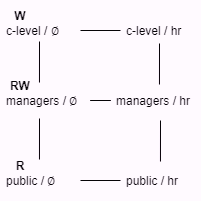
\includegraphics{lattice}

\end{document}
